\section{Keys to to Relativity}

There are two main concepts we need to already touch which are very important for all relativity, from Galilean to General.
These two concepts are not very hard to grasp and if you had a course in Physics or if you followed the lecture notes on Tensor for Beginners 
or Tensor Calculus, you already know.\\

\begin{itemize}
    \item Invariance
    \item Covariance and contravariance
\end{itemize}

The concept of invariance is quite straight forward, and basically means that the same physical objects can be described 
in different ways from different points of view.
Let's take a very simple example of a physical object, a pencil lying on a table.
This pencil can be described using a flat 2D space using the standard orthonormal coordinate system $x$ and $y$, as a vector basically.
This vector can be written as a linear combination of the basis vectors $e_x$ and $e_y$, so practically, its length
can be measured as the sum of a scalar multiplying $e_x$ and another scalar multiplying $e_y$. The scalars are also known as the components  
of this pencil vector, in this coordinate system.\\

Now, imagine we try to describe the same vector (the pencil) using a different coordinate system, which is rotated by some angle with respect to the 
$x$ and $y$ axes, on the same origin.
In this new coordinate system, the vector will have different components, but the vector itself describing the pencil does not change.\\

This is indeed the invariance, so the same object (the pencil i.e. the vector) can be described in different ways when using different coordinate systems (basis vectors).
This is also true for the muon's example of the previous section if you think about that.
In its own reference frame, the muon decays in $2.2 \mu s$, but in Earth's reference frame, the time it takes for his decay is 10 times larger ($\approx 20 \mu s$) due to the time 
dilation effect.\\
This is not very different to explain if we use vectors and the idea of invariance. If we observe the muon creation and its later decay in space-time, the separation
between these two events can be measured using vectors. With the muon coordinate system, this vector is measured to be $2.2 \mu s$, but in another coordinate system, the decay 
time can be measured to be $20 \mu s$. Time dilation in special relativity is really just the result of measuring space-time points using different 
basis vectors.

\begin{center}
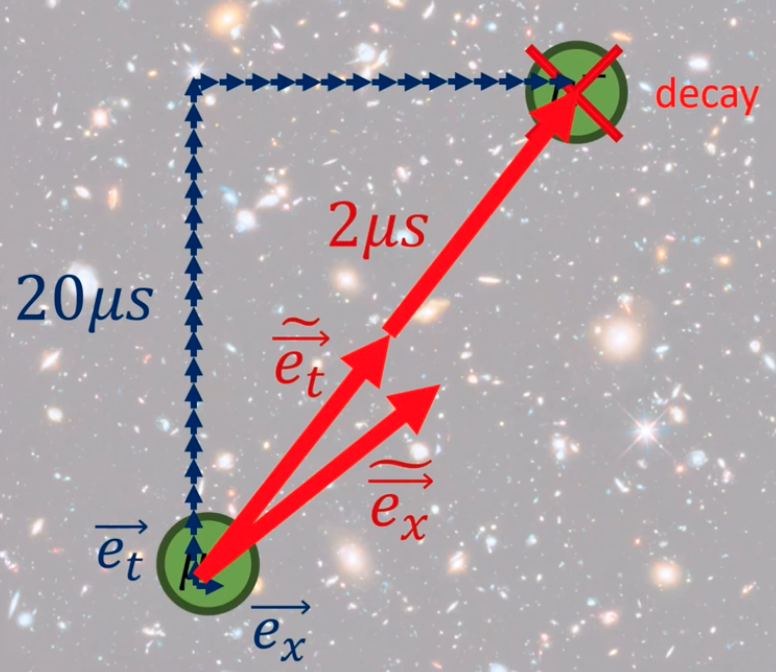
\includegraphics[scale=0.2]{figures/muon-decay.png}
\end{center}

About the concept of covariance and contravariance, they basically mean that, when one thing grows, another thing shrinks, and the opposite
changes will balance out.\\
This concept has been covered thoroughly on the Tensor lecture notes, but let's touch again on this briefly.
When you perform any coordinate transformation, this changes both the basis and the compoents of the vectors described, and these c
change in opposite ways!\\
Vector basis are covariant with change of coordinates, whereas vector components are contravariant.
When basis changes one way, vector's components change in the opposite way.
